% \begin{savequote}[75mm]
% Nulla facilisi. In vel sem. Morbi id urna in diam dignissim feugiat. Proin molestie tortor eu velit. Aliquam erat volutpat. Nullam ultrices, diam tempus vulputate egestas, eros pede varius leo.
% \qauthor{Quoteauthor Lastname}
% \end{savequote}

\chapter{Finding Structure in Functional Networks}


%Hawkes process inference relied on an augmentation strategy 
%made possible by the linear form and excitatory nature 
% of the interactions. In neural settings, these assumptions 
%of the Hawkes process are not as realistic. Instead, we turn to 
%the nonlinear Hawkes process, which allows for both excitatory 
%and inhibitory interactions by introducing a nonlinearity 
%into the model. This corresponds to the popular generalized 
%linear model that is widely used in computational neuroscience. 
%We develop a novel approach that leverages the 
%\polyagamma augmentation to enable efficient, fully-conjugate 
%inference. Again, we combine the nonlinear Hawkes process with 
%prior distributions on the network of interactions, and we focus 
%on a discrete time approximation. This is part of ongoing work 
%with Ryan and Jonathan Pillow at Princeton, and it has grown out 
%of a Cosyne abstract \cite{linderman2015cosyne}. I also have an 
%unpublished draft in which I extend the abstract and apply it 
%to a variety of neural datasets, and show how the network models 
%recover interesting latent features like neural types and locations.
%I will submit a journal version of this paper as soon as possible.

%\section{Abstract} 
%We develop a novel method for the unsupervised discovery of interpretable latent structure underlying neural recordings. 
%Rather than directly clustering or factorizing measured activity, we propose a generative model that links latent clusters and features of neurons to measured activity via an intermediate functional network. 
%Thus, latent structure is defined in terms of how neurons interact with one another rather than how they behave. 
%To discover the most appropriate structural form, we propose a fully-Bayesian inference algorithm that enables efficient inference and principled model comparison. 
%We demonstrate the efficacy of this approach on synthetic data and simultaneously recorded multi-neuronal spike trains.


%\section{Introduction}
With the advent of novel technologies for large-scale recording of
neural activity~\cite{grewe2010high, prevedel2014simultaneous,
  churchland2012neural, holekamp2008fast, ahrens2013whole,
  portugues2014whole, alivisatos2012brain, briggman2005optical,
  ahrens2012brain} there comes a pressing need for methods of
analyzing neural recordings and uncovering their underlying structure.
The goal of these methods is not only to capture variability in
activity and make accurate predictions, but to expose meaningful,
low-dimensional structure that may lead to novel hypotheses and
interpretations of the circuits under study. In other words, we
need \emph{exploratory} methods~\cite{tukey1962future} that yield interpretable
\emph{representations} of large scale data.  
For example, populations of retinal ganglion cells may be represented as a 
set of subpopulations, each performing a distinct
computational role and interacting in characteristic ways with
other subpopulations~\cite{sanes2015types}.
Likewise, some populations may be characterized by continuous features,
like retinotopic location or tuning direction.
As we probe complex circuits far removed from stimuli and behavioral
outputs, we need methods that automatically extract these simplified
representations.

There are a variety of data analysis methods designed to meet this
need.  Relatively simple analyses, like principal components analysis
and k-means clustering, 
%can be performed at scale with distributed computing platforms~\cite{freeman2014mapping}. 
can provide insight into latent features and types of neurons, but they do 
not account for important temporal dynamics of neural activity. 
At the other end of the
spectrum, there are many sophisticated models that explicitly model
temporal dynamics, like generalized linear models~\cite{Truccolo-2005,
  Paninski-2004, Pillow-2008}, state space models~\cite{Smith-2003,
  paninski2010new, Buesing12, escola2011hidden,
  linderman2016nonparametric}, and others~\cite{Yu09,
  churchland2012neural, cunningham2007inferring},
but applying these methods and interpreting their results requires
more expertise. 

We introduce a modeling framework that combines the desirable 
properties of both of these approaches: it captures the autoregressive 
dynamics of neural populations as well as interpretable, high-level 
latent variables that govern those dynamics. The crucial link is 
provided by a structured model for the network of functional 
connections. Probabilistic network models~\cite{Hoff-2002}
describe structure in the pattern of connections and weights in 
terms of neuron-specific latent variables. For example, 
neurons may have latent locations that govern the probability of 
connection or latent types that specify the strength of interaction.
Given the network, we specify an generative model for spike 
trains in which action potentials induce impulse responses on 
downstream neurons that modulate the probability of spiking. 
These autoregressive dynamics are the basis for the popular 
generalized linear model (GLM)~\cite{Truccolo-2005, Paninski-2004, Pillow-2008}
of multineuronal spike trains. 
As we will show, by incorporating these probabilistic network models 
into the GLM, we can recover meaningful 
and interpretable patterns on the basis of neural activity alone.


\begin{figure}[t]
  \centering
  \begin{subfigure}[b]{1.3in}
    \centering
    \caption{}
    \vspace{-.25in}
    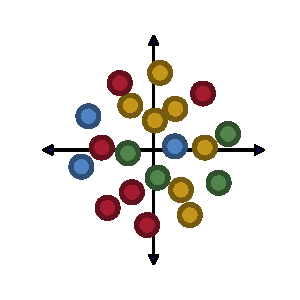
\includegraphics[width=\textwidth]{figures/ch3/new_clustered_embedded_neurons}
    \label{fig:fig1_network}
  \end{subfigure}
   \begin{subfigure}[b]{1.3in}
     \centering
     \caption{}
     \vspace{-.25in}
     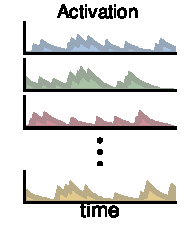
\includegraphics[width=\textwidth]{figures/ch3/new_activation}
     \label{fig:fig1_activation}
   \end{subfigure}
   \begin{subfigure}[b]{1.3in}
     \centering
     \caption{}
     \vspace{-.25in}
     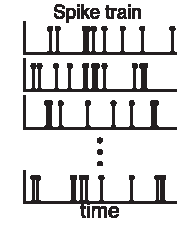
\includegraphics[width=\textwidth]{figures/ch3/new_observed_spikes}
     \label{fig:fig1_spikes}
   \end{subfigure}
   \begin{subfigure}[b]{1.3in}
     \centering
     \caption{}
     \vspace{-.25in}
     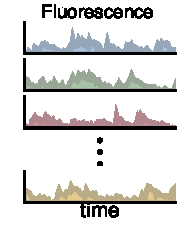
\includegraphics[width=\textwidth]{figures/ch3/new_observed_fluorescence}
     \label{fig:fig1_fluorescence}
   \end{subfigure}
   \vspace{-.2in}
   \caption{Components of the generative model. 
     \textbf{(a)} Each neuron is endowed with latent variables, like 
     locations in space and discrete types (illustrated with different colors).
     These variables determine the probability of connections and the 
     strength of those connections. In this example, nearby neurons of the same 
     type are most likely to connect.
     \textbf{(b)} The network parameterizes an autoregressive model 
     with a time-varying activation, which specifies the instantaneous probability 
     of an action potential.
     \textbf{(c)} Spikes are randomly generated according to the 
     activation. Each spike induces an impulse response on the activation 
     of downstream neurons.
     \textbf{(d)} In imaging studies, we only observe a noisy fluorescence 
     trace that reflects the underlying spike train.}
 \label{fig:fig1}
 \end{figure}

Figure~\ref{fig:fig1} illustrates the components of our generative model. 
In this example, each neuron belongs to one of four classes (\textit{red}, \textit{blue}, \textit{green}, or \textit{yellow}). Additionally, neurons have a latent location in two-dimensional space. The connection probability is determined by distance between the locations (nearby neurons are more likely to connect), as well as the latent types (neurons of the same type are more likely to connect).
This network parameterizes an autoregressive model for neural activity.
The instantaneous probability of firing an action potential is a function of the underlying \textit{activation}.
The activation obeys autoregressive dynamics: when a neuron fires an action potential, an impulse response is added to the activation of downstream neurons. Excitatory connections induce positive impulse responses; inhibitory connections induce negative ones. 
on the \textit{activation} of downstream neurons
In many modern recordings, the spike trains must be inferred from an observed calcium fluorescence trace. In these cases, the model may be augmented with a generative model for fluorescence 
that captures the slower calcium dynamics~\cite{Vogelstein-2010, Mishchenko11a}. 

In our framework, probabilistic network models formalize the intuitive belief 
that functional connections arise from underlying latent variables. 
For some well-studied populations, like retinal ganglion cells (RGCs) 
and hippocampal place cells, 
we already have a strong intuition about what these latent 
variables should be --- RGCs come in a variety of 
distinct types and respond to light in their receptive field, 
while hippocampal place cells reflect locations 
in the environment. These exemplify the interpretable latent variables 
we wish to infer for other brain circuits, 
which have eluded simplifying representations. 

% This generative approach formalizes many of the intuitive hypotheses already employed in neuroscience. 
% Neural circuits are commonly described with simplified block diagrams that show how one subpopulation of neurons drives another. 
% In other cases, neurons are described by continuous features, such as ``place fields'' that describe the spatial location in which hippocampal place cells fire.
% Since our movement is continuous, neurons with similar place fields are functionally correlated.
% Our approach begins with high-level hypotheses like, ``neurons have latent types that determine functional connectivity.''
% These hypotheses are instantiated as generative models which are then fit to the data using probabilistic inference techniques and compared on the basis of how well they explain the measured activity.

To perform this inference, we develop novel a Markov chain Monte Carlo (MCMC)
algorithm that can efficiently invert this generative procedure 
to explore the posterior distribution over 
latent variables given observed spike trains or calcium fluorescence traces. 
Since we do not know \textit{a priori} what types of latent variables to expect, 
we show how a wide range of hypotheses can be encoded as prior distributions 
over networks. Since weighted, directed networks can be equivalently represented 
as sparse matrices, prior distributions over the space networks correspond 
to distributions over matrices. Specifically, a network can be represented 
as the elementwise product of a real-valued weight matrix~$bW$, whose 
entries~$W_{n \from m}$ specify the strength of the directed connection from 
neuron~$m$ to neuron~$n$, and a binary adjacency matrix~$\bA$, whose 
entries denote whether or not a connection is present. Thus,~$\bA$ specifies 
the sparsity of the network, while~$\bW$ specifies the strength. This 
decomposition is known as a spike-and-slab model in machine 
learning~\cite{Mitchell1988}.

% Network models
\begin{figure}[t!]
  \centering
  \textit{~~~~~Adjacency Model} \\
  % Gaussian row
  \hspace{1em}
  \begin{subfigure}[b]{1.25in}
    \centering
    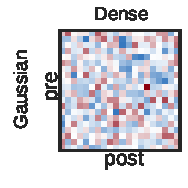
\includegraphics[width=\textwidth]{figures/ch3/Dense-Gaussian.pdf}
  \end{subfigure}
  ~
  \begin{subfigure}[b]{1.10in}
    \centering
    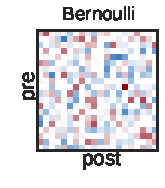
\includegraphics[width=\textwidth]{figures/ch3/Bernoulli-Gaussian.pdf}
  \end{subfigure}
  ~
  \begin{subfigure}[b]{1.10in}
    \centering
    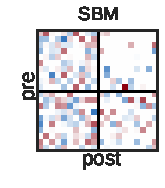
\includegraphics[width=\textwidth]{figures/ch3/SBM-Gaussian.pdf}
  \end{subfigure}
  ~
  \begin{subfigure}[b]{1.10in}
    \centering
    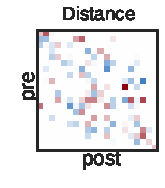
\includegraphics[width=\textwidth]{figures/ch3/Distance-Gaussian.pdf}
  \end{subfigure}
  \\
  % SBM row
  \rotatebox{90}{\textit{~~~~~Weight Model}}
  \begin{subfigure}[b]{1.25in}
    \centering
    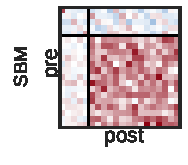
\includegraphics[width=\textwidth]{figures/ch3/Dense-SBM.pdf}
  \end{subfigure}
  ~
  \begin{subfigure}[b]{1.10in}
    \centering
    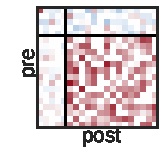
\includegraphics[width=\textwidth]{figures/ch3/Bernoulli-SBM.pdf}
  \end{subfigure}
  ~
  \begin{subfigure}[b]{1.10in}
    \centering
    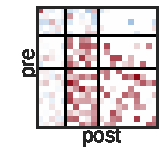
\includegraphics[width=\textwidth]{figures/ch3/SBM-SBM.pdf}
  \end{subfigure}
  ~
  \begin{subfigure}[b]{1.10in}
    \centering
    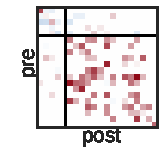
\includegraphics[width=\textwidth]{figures/ch3/Distance-SBM.pdf}
  \end{subfigure}
  \\
  % Distance row
  \hspace{1em}
  \begin{subfigure}[b]{1.25in}
    \centering
    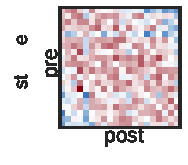
\includegraphics[width=\textwidth]{figures/ch3/Dense-Distance.pdf}
  \end{subfigure}
  ~
  \begin{subfigure}[b]{1.10in}
    \centering
    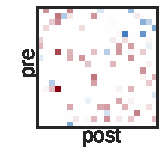
\includegraphics[width=\textwidth]{figures/ch3/Bernoulli-Distance.pdf}
  \end{subfigure}
  ~
  \begin{subfigure}[b]{1.10in}
    \centering
    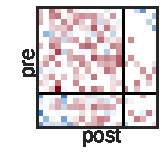
\includegraphics[width=\textwidth]{figures/ch3/SBM-Distance.pdf}
  \end{subfigure}
  ~
  \begin{subfigure}[b]{1.10in}
    \centering
    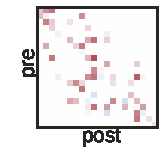
\includegraphics[width=\textwidth]{figures/ch3/Distance-Distance.pdf}
  \end{subfigure}
  \caption{Example network models. Each row corresponds to a fixed weight matrix,~$\bW$, 
    and each column corresponds to a fixed adjacency matrix,~$\bA$. The panels show 
    the elementwise product of the two. In the left column, the adjacency matrix is 
    dense, i.e.~$A_{n \from m} \equiv 1$ for all pairs. Thus the left column shows
    just the matrix~$\bW$. Color denotes the weight (blue is negative, red is postiive).
    The second column shows an independent Bernoulli adjacency 
    model in which each connection is present with the same probability. In the SBM, 
    each neuron has a latent cluster assignment that governs the probability of 
    connections, and in the distance model, the neurons have a latent location such 
    that nearby neurons are more likey to connect. In the SBM, the rows and columns 
    are sorted by type, and in the distance model, they are sorted by location. 
    In the top row, the weights are drawn from an independent Gaussian model. The 
    SBM has type-dependent mean weights. The distance model has weights that 
    decrease as a function of distance, whcih leads to the banded structure.
    independent Gaussian model}
  \label{fig:network_models}
\end{figure}

Figure~\ref{fig:network_models} shows how a variety of networks can be 
constructed by combining different priors on the weights 
(rows) with priors on the pattern of 
connectivity (columns). Each row corresponds to a fixed weight matrix 
drawn from a independent Gaussian prior, a stochastic block model (SBM), or a latent 
distance model. Each column corresponds to a fixed adjacency matrix 
drawn from a complete graph model, and independent Bernoulli model, 
an SBM, or a latent distance model. The matrices show the elementwise 
product, which encodes a weighted, directed network. Standard generalized linear models implicitly assume a complete network with 
independent Gaussian weights (top left panel of Figure~\ref{fig:network_models}).
Here, all pairs of neurons are connected to each other and all weights are 
independent, identically distributed Gaussian random variables. By using latent variable 
models, we can construct much richer network models in which the sparsity 
and strength of connections depend on types and locations of neurons. 
Complete details of these models are given in Section~\ref{sec:methods}

Once we have specified a class network models, we can perform inference and 
evaluate them on the basis of their predictive power. A good model should 
be able to generalize to new neurons by predicting the neurons' latent 
variables and connections. If these predictions are accurate, the model 
will assign high probability to the held-out neurons' spike trains. 
In this way, we can assess the quality of the different network models
and determine which latent variable model is most appropriate for the 
neural population under study. This provides a flexible, data-driven 
method of exploring a variety of hypotheses about interpretable structure 
underlying complex, dynamical models of neural activity.


\section{Results}
We demonstrate the efficacy of this approach by applying our framework 
to two neural populations for which we have longstanding experimental 
evidence in favor of a particular latent variable representation.
First, we consider a population of simultaneously recorded retinal 
ganglion cells (RGCs), which can be characterized by their type 
(either \textit{on} or \textit{off} in this dataset) and
by the location of their receptive field centers. 
We then consider a population of hippocampal place cells, which encode 
positions in a two dimensional environment. In both cases, our approach 
recovers these latent representations given only the neural spike trains,
without any knowledge of the stimulus or the true location.

\subsection{Retinal Ganglion Cells}

\begin{figure}[t!]
  \centering
  \begin{subfigure}[b]{2.25in}
    \centering
    \caption{}
    \vspace{-.2in}
    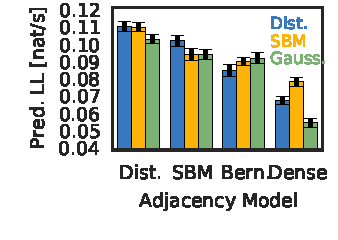
\includegraphics[width=\textwidth]{figures/ch3/rgc_pred_ll_bar.pdf}
    \label{fig:rgc_pll}
  \end{subfigure}
  ~
  \begin{subfigure}[b]{1.6in}
    \centering
    \caption{}
    \vspace{-.2in}
    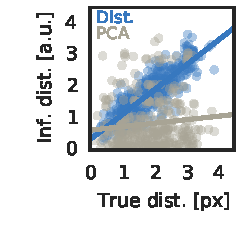
\includegraphics[width=\textwidth]{figures/ch3/rgc_pairwise_distance_scatter.pdf}
    \label{fig:rgc_dist}
  \end{subfigure}
  ~
  \begin{subfigure}[b]{1.6in}
    \centering
    \caption{}
    \vspace{-.2in}
    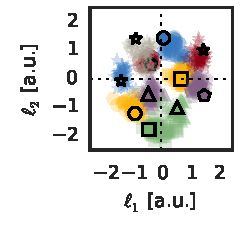
\includegraphics[width=\textwidth]{figures/ch3/rgc_on_locations.pdf}
    \label{fig:rgc_locs}
  \end{subfigure}
  \\
  \vspace{-.2in}
  \begin{subfigure}[b]{1.85in}
    \centering
    \caption{}
    \vspace{-.2in}
    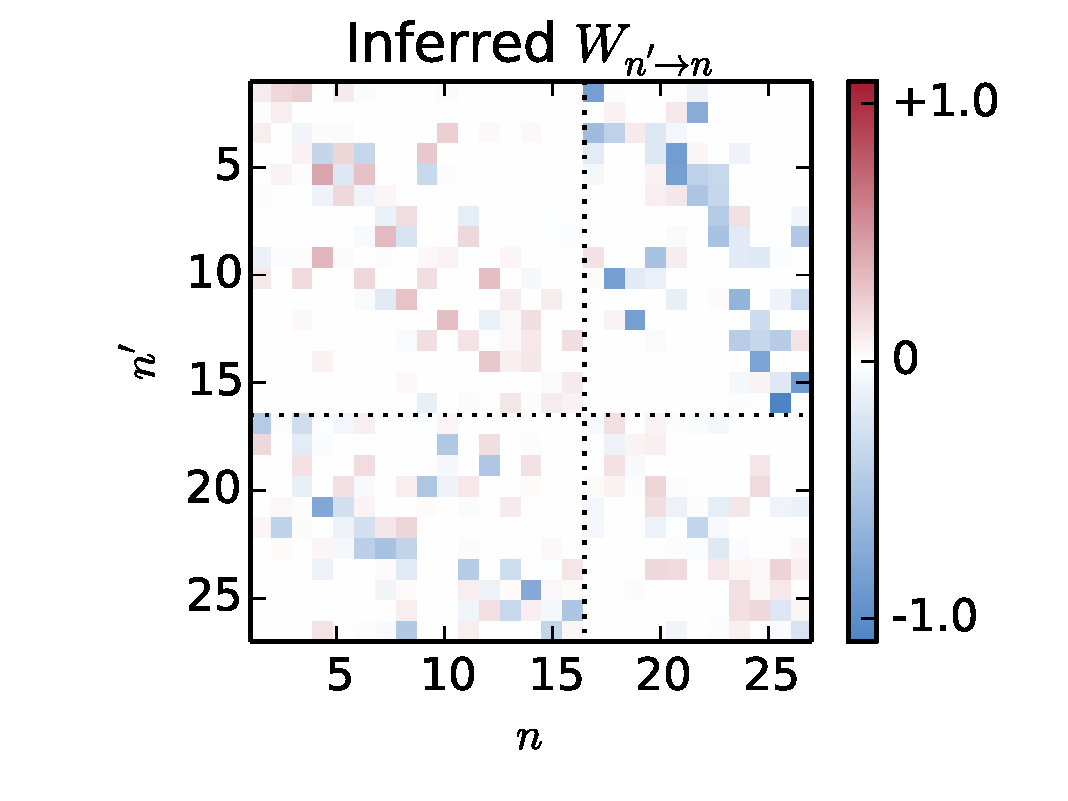
\includegraphics[width=\textwidth]{figures/ch3/rgc_connectivity.pdf}
    \label{fig:rgc_w}
  \end{subfigure}
  ~
    \begin{subfigure}[b]{1.85in}
    \centering
    \caption{}
    \vspace{-.2in}
    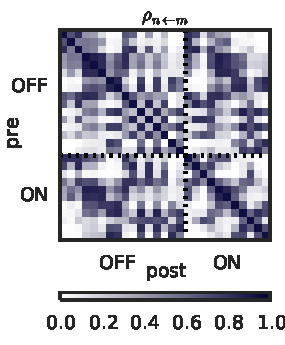
\includegraphics[width=\textwidth]{figures/ch3/rgc_prob_conn.pdf}
    \label{fig:rgc_rho}
  \end{subfigure}
  ~
  \begin{subfigure}[b]{1.85in}
    \centering
    \caption{}
    \vspace{-.2in}
    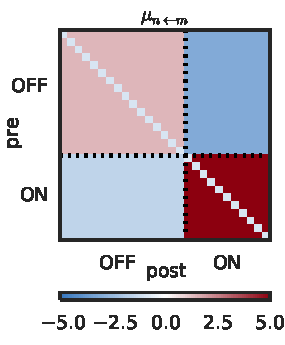
\includegraphics[width=\textwidth]{figures/ch3/rgc_mean_conn.pdf}
    \label{fig:rgc_mu}
  \end{subfigure}
  \vspace{-2em}
  \caption{Retinal ganglion cell types and locations can be inferred
    from spike trains alone.
    \textbf{(a)} The combined distance model and block model yields the highest predictive log likelihood (units: nats/spike), compared to other combinations of adjacency models (groups of bars) and weight models (\textit{blue}: latent distance weight model, \textit{yellow}: stochastic block model for weights, \textit{green}: Gaussian weights).
    \textbf{(b)} The inferred distances under the latent distance model are highly correlated with the true distances, as measured by stimulus sensitivity, whereas inferred embeddings under PCA are not.
    \textbf{(c)} Moreover, the inferred locations (semitransparent markers) recover the true receptive field centers (solid markers with black outline). Shown here only for ON cells.
    \textbf{(d)} Inferred network,~${\bA \odot \bW}$, under a latent distance model of connection probability and a stochastic block model for connection weight, averaged over 500 posterior samples.
    \textbf{(e)} Expected probability of connection under the latent distance model.
    \textbf{(f)} Expected connection strength under the stochastic block model. The inferred cell classes perfectly match the true ON and OFF types, and reflect within-class excitation and between-class inhibition.
}
  \label{fig:rgc}
\end{figure}

We applied our model to simultaneously recorded multineuronal spike
trains from a population of 27 primate retinal ganglion cells
(RGCs). This dataset was previously analyzed with a generalized linear
model in \cite{Pillow-2008}.  In this
dataset, the population is presented with a Gaussian white noise video
with pixel sizes tuned to approximately the width of a receptive
field. We trained our models on one minute of spiking activity, binned at 1ms time
resolution. There were approximately 50,000 spikes in this recording.
We also held out one minute of data for model evaluation.

Retinal ganglion cells respond to light (or the absence thereof) shown
upon their receptive field. The cells are roughly evenly distributed
across the two-dimensional retinal plane. Thus, it is natural to
characterize these cells by the location of their receptive field
center.  Moreover, this population is comprised of two types of cells,
\textit{on} and \textit{off} cells, characterized by their response to
visual stimuli. \textit{On} cells increase their firing when light is
shone upon their receptive field; \textit{off} cells decrease their
firing rate in response to light in their receptive field.  Cell types
are identified by similarity in their response properties as well as
morphological and physiological properties~\cite{sanes2015types}. With
knowledge of the stimulus, these cells can be clearly separated into
their respective types by clustering the spike-triggered average
simulus.  This characterization in terms of latent locations and cell
types has been validated through decades of experiments, and has been
made possible by the relative ease with which relevant stimuli can be
identified and controlled. To what extent can these latent
representations be discovered from the spike trains alone?

We fit our model to the measured spike trains for each of the twelve
probabilistic network priors shown above --- three weight models and
four adjacency models. Predictive likelihood comparisons on the
held-out data reveal that the adjacency matrix, i.e. the pattern of
connectivity, is well-characterized by a two-dimensional latent
distance model (Fig.~\ref{fig:rgc_locs}, as expected given the
localized receptive fields of RGCs. Moreover, the pairwise distances
between the latent locations are highly correlated with the true
distances between receptive field centers (Fig.~\ref{fig:rgc_dist}),
even though the stimulus was never used during training. By contrast,
the inferred locations given by the top two principal components of
the spike trains are highly uncorrelated, indicating that PCA does not
recover a meaningful spatial embedding.  Finally, the inferred
locations can be rotated and scaled such that they match the true
locations almost perfectly (Fig.~\ref{fig:rgc_locs}). Rotation does
not change the pairwise distances and scaling simply changes the
units. This matching is highly unlikely for randomly distributed
locations.  In Fig.~\ref{fig:rgc_locs}, the true locations are shown
as solid markers with black outlines, and the inferred locations
sampled from the posterior distribution are shown as semitransparent
markers of the same color and shape.

For the weight matrix, a latent distance model (Dist) and a stochastic
block model (SBM) both yield similar predictive likelihoods. Looking
into the inferred types under the SBM, we find that the neurons are
grouped according to their true \textit{on} and \textit{off} cells,
again without any knowledge of the stimulus. These types determine 
the expected interaction weight for each pair of neurons. 

\TODO{Compare this to kmeans clustering on the spike train?}

Figure~\ref{fig:rgc_w} shows the inferred functional network under the
latent distance adjacency model and stochastic block model for
weights.  The neurons are sorted first by their type (\textit{off}
then \textit{on}) and then by their $x$-location. This yields the
three bands in the matrix of connection
probabilities~\ref{fig:rgc_rho}. Nearby cells have much higher
probability of connection. The mean connection strength
(Fig.~\ref{fig:rgc_mu}) shows the characteristic pattern of positive
weights between cells of the same type and negative weights betewen
cells of opposite types. The diagonal of this matrix shows the weights
of self-connections, which are typically negative due to refractory
effects. 

Together, these inferred types and locations provide 
compelling evidence for a highly structured pattern of functional 
connectivity. Given the extensive work on characterizing retinal 
ganglion cell responses, we have considerable evidence that the 
representation we learn from spike trains alone is indeed the 
optimal way to characterize this population of cells. This 
lends us confidence that we may trust the representations learned from 
spike trains recorded from deeper brain areas, where traditional 
stimulus-response correlations are less valuable.

\subsection{Hippocampal Place Cells}


\begin{figure}[t!]
  \centering
  \vspace{-.2in}
  \begin{subfigure}[b]{1.75in}
    \centering
    \caption{}
    \vspace{-.2in}
    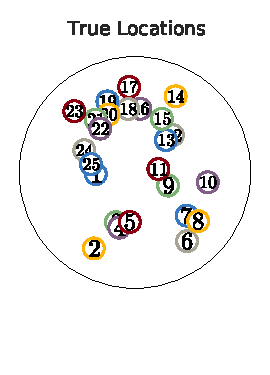
\includegraphics[width=\textwidth]{figures/ch3/hipp_true_locations.pdf}
    \label{fig:hipp_true_locs}
  \end{subfigure}
  ~
  \begin{subfigure}[b]{1.75in}
    \centering
    \caption{}
    \vspace{-.2in}
    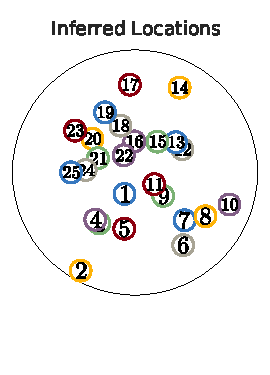
\includegraphics[width=\textwidth]{figures/ch3/hipp_inferred_locations.pdf}
    \label{fig:hipp_inf_locs}
  \end{subfigure}
  ~
  %\begin{subfigure}[b]{1.75in}
  %  \centering
  %  \caption{}
  %  \vspace{-.2in}
  %  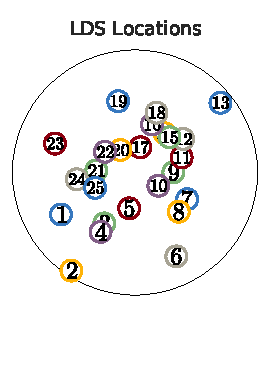
\includegraphics[width=\textwidth]{figures/ch3/hipp_lds_locations.pdf}
  %  \label{fig:hipp_lds_locs}
  %\end{subfigure}
  %\\
  %\vspace{-.2in}
  \begin{subfigure}[b]{1.75in}
    \centering
    \caption{}
    \vspace{-.2in}
    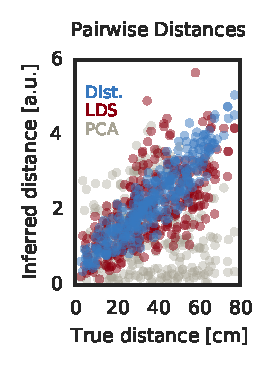
\includegraphics[width=\textwidth]{figures/ch3/hipp_pairwise_distance_scatter.pdf}
    \label{fig:hipp_distances}
  \end{subfigure}
  %~
  \\
  \vspace{-.2in}
  \begin{subfigure}[b]{2.25in}
    \centering
    \caption{}
    \vspace{-.2in}
    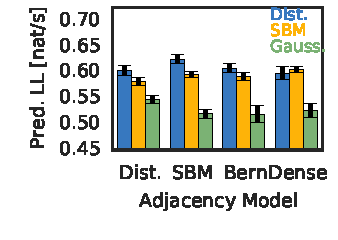
\includegraphics[width=\textwidth]{figures/ch3/hipp_pred_ll_bar.pdf}
    \label{fig:hipp_pll}
  \end{subfigure}
  ~
  \begin{subfigure}[b]{1.85in}
    \centering
    \caption{}
    \vspace{-.2in}
    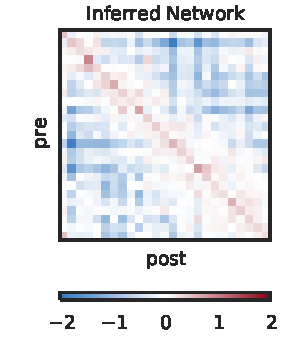
\includegraphics[width=\textwidth]{figures/ch3/hipp_connectivity.pdf}
    \label{fig:hipp_conn}
  \end{subfigure}
  \vspace{-2em}
  \caption{Hippocampal place fields are inferred from population spike trains.
    }
  \label{fig:hipp}
\end{figure}

We also applied our framework to simultaneously recorded multi-neuronal spike trains from the hippocampus of freely moving rats in a circular arena. 
%Experiments were conducted under the supervision of the Massachusetts Institute of Technology (MIT)  Committee on Animal Care and followed the NIH guidelines.
%The micro-drive arrays containing multiple tetrodes were implanted above the  right dorsal hippocampus of male Long-Evans rats. 
%The tetrodes were slowly lowered into the brain reaching the cell layer of CA1 two to four weeks following the date of surgery. 
%Recorded spikes were manually clustered and sorted.
This dataset consists of~$N=25$ neurons recorded for a duration of almost ten minutes and binned in 250ms time bins.
The rat is freely foraging in an open field enviornment roughly 120cm in diameter.
%Since place cells are primarily active during location, the spike train is segmented into individual running epochs by discarding bins in which the velocity is less than 10cm/s. 
%This results in a dataset that is approximately 2000 time bins in length.

As in the retina, we have strong intuitions about the latent structure underlying hippocampal place cell activity, namely, we expect cells representing nearby locations to be correlated and cells with disjoint place fields to be anticorrelated. Can we extend the spatial layout of place fields from spike trains alone?

We apply our framework, fitting all twelve network models and
evaluating them on the basis of predictive likelihood. In this case,
the distance dependent weight models yield the highest predictive
likelihood (Fig.~\ref{fig:hipp_pll}). The stochastic block model
yields the highest predictive likelihood, but upon futher
investigation we find that almost all neurons are connected in this
model. There is one outlier, neuron \#1, which is only sparsely
connected. The SBM assings 24 neurons are assigned to one cluster, and
assigns neuron \#1 to its own group. \TODO{Put this figure in the supplementary material}
Thus, the stochastic block model is quite similar to an independent
Bernoulli model, as is evident from the similar predictive likelihood 
of these two models. 

Looking into the inferred locations under the latent distance model
for the weight matrix, we find that the inferred locations
(Fig~\ref{fig:hipp_inf_locs}) are, up to rotation and scale, highly
similar to the true place field centers (Fig~\ref{fig:hipp_true_locs})
measured using the rat's true location. This is quantified by 
plotting the pairwise distances between inferred locations against 
the pairwise distances between place field centers. The latent 
distance model's pairwise distances are highly correlated with the 
ground truth, whereas distances between PCA embeddings are very uncorrelated (Fig.~\ref{fig:hipp_distances}). For further comparison, we fit a Poisson linear dynamical system (PLDS) \cite{macke2011empirical} with a two dimensional latent state space, and used the rows of the 
~$N \times 2$ emission matrix as the locations of the neurons. This sophisticated 
model, which captures temporal dynamics of the neural population, yields 
pairwise distances that are quite correlated with the true distances, 
but we find that the variance of this fit grows with the true distance.
This reflects the fact that the PLDS does not explicitly parameterize
interaction as a function of distance, but rather induces correlation 
due to similarity in the emission matrix as well as shared dynamics.

Finally, we investigated the expected network under the posterior and 
found that upon sorting the neurons by their inferred locations, an
intuitive banded structure emerges (Fig.~\ref{fig:hipp_conn}). 
The positive diagonal indicates strong autocorrelation between a 
neurons spiking in consecutive 250ms bins. Over these time scales, 
self-refractory effects are not evident. The primary connections 
are inhibitory in nature, such that active cells suppress the activity 
of cells with distal place fields. 

These inferred representations again confirm our intuitive beliefs 
about the structure of hippocamapl place cell responses. The 
inferred latent variables recover meaningful structure in the
neural activity, without any access to the location. Instead, 
these representations arise from the neural activity alone.

\subsection{Synthetic Data}

\TODO{
How scalable is this approach?
When would simpler methods suffice?
Could we just fit a GLM and then model its weights?
}

\section{Methods}
\label{sec:methods}
Our primary contribution is a novel framework for discovering latent
network structure underlying neural activity.  This framework consists
of a probabilistic model relating structure to observed signals, an
efficient Bayesian inference algorithm capable of fitting this model,
and a model selection algorithm that enables principled comparison of
structural forms.

\subsection{Probabilistic Model}
A probabilistic model specifies a joint probability distribution over
measured signals, the underlying network, and latent structural
variables we wish to infer.  In our model, the measured signal from
neuron~$n$ in the~$t$-th time bin is denoted~$s_{t,n}$, which may 
denote either a discrete spike count or a real-valued signal, like 
the calcium fluorescence. In either case, this signal is assumed 
to be stochastically drawn from a distribution parameterized by 
an underlying, real-valued \emph{activation},~$\psi_{t,n}$,
and a static parameter,~$\nu_n$. The
activation is typically related to the expected spike count via
a logistic transformation,~$\sigma(\psi) = e^\psi \, (1+e^\psi)^{-1}$,
which has the property~$\sigma(-\psi) = 1-\sigma(\psi)$.

\begin{table}
\begin{center}
\begin{tabular}{c|c|c|c|c}
  \textbf{Distribution} & $p(s \given \psi, \nu)$ & Standard Form & $\bbE[s]$ & $\Var(s)$ \\
  \hline
  Gaussian & $\frac{1}{\sqrt{2 \pi \nu}}\exp \left \{ -\frac{1}{2 \nu} (s - \psi)^2 \right \}$
  & --- 
  & $\psi$ & $\nu$ \\
  Bernoulli & $\sigma(\psi)^s \, \sigma(-\psi)^{1-s}$
  & $\frac{(e^\psi)^s}{1+e^\psi}$
  & $\sigma(\psi)$ & $\sigma(\psi) \, \sigma(-\psi)$ \\
  Binomial & ${\nu \choose s} \, \sigma(\psi)^s \, \sigma(-\psi)^{\nu-s}$
  & ${\nu \choose s} \,\frac{(e^\psi)^s}{(1+e^\psi)^\nu}$
  & $\nu \sigma(\psi)$ & $\nu \sigma(\psi) \, \sigma(-\psi)$ \\
  Neg. Binomial & ${\nu + s -1 \choose s} \, \sigma(\psi)^s \, \sigma(-\psi)^{\nu}$
  & ${\nu +s - 1 \choose s} \,\frac{(e^\psi)^s}{(1+e^\psi)^{\nu+s}}$
  & $\nu e^\psi$ & $\nu e^\psi / \sigma(-\psi)$ \\
\end{tabular}
\end{center}
\caption{List of observation distributions.}
\label{tab:obs_models}
\end{table}

We consider the four observation models shown in Table~\ref{tab:obs_models}.
The Gaussian model assumes~$s_{t,n}$ is real-valued, and may be
appropriate for modeling calcium fluorescence, for example.
The Bernoulli distribution is appropriate for binary spike counts,
whereas the binomial and negative binomial have support
for~$s\in[0,\nu]$ and~$s \in [0, \infty)$, respectively.
Notably lacking from this list is the Poisson distribution,
which does not seem to be amenable to the augmentation schemes
we will derive below. Nevertheless, both the binomial and negative
binomial distributions converge to the Poisson under certain
limits, and they afford the added flexibility of modeling under- and
over-dispersed spike counts. Specifically, while the Poisson has unit 
dispersion (its mean is equal to its variance), the binomial distribution 
is always under-dispersed, since its mean always exceeds its variance, 
and the negative binomial is always over-dispersed, with variance greater 
than its mean.

The generalized linear model (GLM) \cite{Paninski-2004, Truccolo-2005, Pillow-2008} 
models the activation at time~$t$ as a weighted function of 
the spike counts at preceding times~${[0,t-1]}$. Specifically,
let,
\begin{align}
  \label{eq:glm_activation}
  \psi_{t,n} &\triangleq w_n^{(0)}  +                 
               \sum_{m=0}^N  \sum_{k=1}^K a_{n \from m} \, w_{n \from m}^{(k)}
               \left( \sum_{\Delta t=1}^{\Delta t_{\mathsf{max}}} \phi_{k, \Delta t} \cdot s_{t-\Delta t, m} \right) \\
             &= w_n^{(0)}  + \sum_{m=0}^N \sum_{k=1}^K a_{n \from m} \, w_{n \from m}^{(k)} \, \widehat{s}_{t,m}^{(k)} \\
  \label{eq:linear_activation}
             &= (\ba_{n} \odot \bw_n)^\trans \, \widehat{\bs}_t,
\end{align}
where~$w_n^{(0)}$ is the baseline activation of neuron~$n$,
$\bphi_{k,1:\Delta t_{\mathsf{max}}}$ is a basis function 
that weights the previous spike counts for 
offsets~${\Delta t \in [1, \Delta t_{\mathsf{max}}]}$
, the binary variable~${a_{n \from m} \in \{0,1\}}$ 
indicates whether or not there exists 
a directed connection from neuron~$m$ to neuron~$n$,
and~$w_{n \from m}^{(k)}$ captures the influence that
spikes on neuron~$m$ exert on neuron~$n$ at
offsets weighted by the~$k$-th basis function.  
Since the basis function and the signal 
are assumed to be fixed,  can precompute the inner sum, which is simply the 
convolution of the signal with the basis function, to get~$\widehat{s}_{t,m}^{(k)}$.
Since this is a linear function, we can combine the
connections, weights, and filtered spike trains into
vectors to get the linear form  in Eq.~\ref{eq:linear_activation}.
Here, we have,
\begin{align}
  \ba_n &=
    \bigg[
      1,  
      &a_{n \from 1}, & & \ldots, & & a_{n \from 1}, 
      & & \ldots, &
      &a_{n \from N}, & & \ldots, & &a_{n \from N} 
    &\bigg]^\trans, \\
  \bw_n &=
    \bigg[
      w_n^{(0)}, 
      &w_{n \from 1}^{(1)}, & & \ldots, & &w_{n \from 1}^{(K)}, 
      & &\ldots, &
      &w_{n \from N}^{(1)}, & & \ldots, & &w_{n \from N}^{(K)} 
      &\bigg]^\trans, \\
  \widehat{\bs}_t &=
    \bigg[
      1, 
      &\widehat{s}_{t,1}^{(1)}, & & \ldots, & &\widehat{s}_{t,1}^{(K)}, 
      & &\ldots, &
      &\widehat{s}_{t,N}^{(1)}, & & \ldots, & &\widehat{s}_{t,N}^{(K)} 
    &\bigg]^\trans,
\end{align}
and~$\odot$ dentoes the elementwise product. For convenience, we
let~$\bA$ and~$\bW$ refer to the~$N \times NK+1$ matrices obtained
by stacking the vectors~$\ba_n^\trans$ and~$\bw_n^\trans$, and we
let~$\widehat{\bS}$ denote the~$T \times NK+1$ matrix with rows
given by~$\widehat{\bs}_t^\trans$. The major difference between this formulation and that of the standard 
GLM is that here we have explicitly modeled the sparsity of the 
weights via the ``adjacency matrix'' $\bA$. Under the standard 
formulation, all weights are present, that is,~${a_{n \from m} \equiv 1}$.

Consider a model with one basis function ($K=1$) defined
by,~${\phi_{1,\Delta t} = e^{-\Delta t/\tau}}$.
Then~$\widehat{s}_{t,m,1}$ is a weighted sum of spikes in the
window~$[t-\Delta t_{\mathsf{max}},t-1]$, where the weights decay
according to an exponential function with time constant~$\tau$.  
If~${A_{n \from m}=1}$, indicating a
connection from neuron~$m$ to neuron~$n$, and
the weight,~$W_{n \from m,1}$, is positive, the influence will be
excitatory. If it is negative, the effect will be inhibitory.
Together, the weights~$\bW$ define a functional \emph{network} of
interactions.

The popularity of generalized linear models is due, in large part, to
the intuitive appeal of networks as a description of neuronal
dynamics.  While the weights of the GLM may not necessarily correspond
to direct synaptic connections, they provide an interpretable
representation of firing rate dynamics in terms of a functional
network. However, this interpretability is hampered by the fact that
there are~$O(N^2)$ weights to reason about, and as the number of
neurons,~$N$, grows, it becomes impossible to make sense of the entire
network.

We extend our probabilistic model with hierarchical latent variable
models that capture intuitive structure in the network, while
retaining the interpretable network-based representation that makes
the GLM so popular. We assume that each neuron is endowed with a set
of latent features that govern the probability of functional
interactions. Specifically, we consider two types of features:
discrete classes,~$c_n \in \{1, \ldots, C\}$, and continuous
locations,~$\bell_n \in \reals^D$. These can determine either the
probability of connection,~$\rho_{n \from m}$, or the mean and
variance of a multivariate Gaussian prior on the
weights,~$\bmu_{n \from m}$ and~$\bSigma_{n \from m}$.
Conditioned upon these latent variables, the connections and 
their weights are all conditionally independent of one another.
That is,
\begin{align}
  p(\ba_n, \bw_n \given c_n, \bell_n, \theta) = 
  p(\ba_n \given c_n, \bell_n, \theta) \, p(\bw_n \given c_n, \bell_n, \theta),
\end{align}
where
\begin{align}
  p(\ba_n \given c_n, \bell_n, \theta) 
  &= \prod_{m=1}^N \distBernoulli(a_{n \from m} \given \rho_{n \from m}), \\
  p(\bw_n \given c_n, \bell_n, \theta) 
  &= \distNormal(w_n^{(0)} \given \mu_0, \sigma^2_0 ) \prod_{m=1}^N 
     \distNormal(\bw_{n \from m} \given \bmu_{n \from m}, \, \bSigma_{n \from m}), \\
  &= \distNormal(\bw_n \given \bmu_n, \bSigma_n).
\end{align}
Here, we have combined the Gaussian factors into single multivariate Gaussian prior
with parameters,
\begin{align}
  \bmu_n 
    &= \begin{bmatrix}
      \mu_0 \\
      \bmu_{n \from 1} \\
      \vdots \\
      \bmu_{n \from N}
    \end{bmatrix}, & \text{ and } & &
  \bSigma_n 
  &= \begin{bmatrix}
    \sigma_0^2 &                     &        & \\
               & \bSigma_{n \from 1} &        & \\
               &                     & \ddots & \\
               &                     &        & \bSigma_{n \from N} 
    \end{bmatrix}.
\end{align}
As previously mentioned, the parameters~$\rho_{n \from m}$,~$\bmu_{n \from m}$, and~$\bSigma_{n \from m}$ 
may depend on~$c_n$,~$\bell_n$, and the parameters of the model,~$\theta$.
The form of these dependencies is a function of the underlying models, 
which we describe next.

\begin{table}
\begin{center}
\begin{tabular}{c|c|c}
Name & Latent Variable & $p(A_{n \from m≈})$ \\
\hline
Dense Model & --- & $1$ \\
Bernoulli Model & --- & $\rho$ \\
Stochastic Block Model & $c_n$ & $\rho_{c_n \from c_m}$ \\
Latent Distance Model & $\bell_n$ & $\sigma(-||\ell_n - \ell_m||_2^2 + \gamma_0)$
\end{tabular}
\end{center}
\caption{Binary Adjacency Matrix Models}
\label{tab:A_models}
\end{table}

Table~\ref{tab:A_models} defines the four adjacency models considered 
herein. The dense model corresponds to the standard GLM in which all
connections are present. The Bernoulli model is a spike-and-slab model 
in which each connection is an independent and identically distributed 
Bernoulli random variable with probability~$\rho$. This is also known 
as an Erd\"os-R\'enyi model. In the stochastic block model (SBM) 
\cite{Nowicki-2001}, the probability of connection depends on the class 
of the up and downstream neurons. The class assignments are drawn from
a categorical prior,~${c_n \sim \distCategorical(\bpi)}$, and the class
weights are given a conjugate, symmetric 
Dirichlet prior,~${\bpi \sim \distDirichlet(\alpha \bone_C)}$. The 
connection probabilities are given a conjugate beta 
prior,~${\beta_{c \from c'} \sim \distBeta(\alpha, \beta)}$. 
The latent distance model \cite{Hoff-2008} encodes the belief that 
connection probability should decrease with distance between latent 
locations. The locations are given spherical Gaussian 
priors,~$\bell_n \sim \distNormal(0, \eta \bI)$, and the scale is
drawn from an inverse gamma prior,~$\eta \sim \distInvGamma(1,1)$. The 
offset is given a standard normal prior,~$\gamma_0 \sim \distNormal(0, 1)$.


\begin{table}
\begin{center}
\begin{tabular}{c|c|c|c}
Name & Latent Variable & $\bmu_{n \from m}$ & $\bSigma_{n \from m}$\\
\hline
Gaussian Model & --- & $\bmu$ & $\bSigma$ \\
Stochastic Block Model & $c_n$ & $\bmu_{c_n \from c_m}$ & $\bSigma_{c_n \from c_m}$ \\
Latent Distance Model (${K=1}$) & $\bell_n$ & $-||\bell_n - \bell_m||_2^2 + \mu_0$ & $\sigma^2$
\end{tabular}
\end{center}
\caption{Gaussian Weight Models}
\label{tab:W_models}
\end{table}

Table~\ref{tab:W_models} defines the three weight models we
consider.  Each model defines the mean and variance of a multivariate
normal distribution,~$\bw_{n \from m} \sim \distNormal(\bmu_{n \from
  m}, \bSigma_{n \from m})$.  In the Gaussian model, all weights are
independent and identically distributed.  The stochastic block model,
has parameters for each pair of classes, each drawn from a normal
inverse-Wishart prior,~$(\bmu_{c \from c'}, \bSigma_{c \from c'}) \sim
\distNormalInvWishart(\mu_0, \kappa_0, \Sigma_0, \nu_0)$. Finally, we
consider a latent distance model, but only for the case where the
weights are scalar, i.e.~$K=1$. In this case, the distance between
points is inversely proportional to the mean weight.  For higher order
weights, additional assumptions would be required in order to relate
distance to vector weights. In this model, we assume standard normal
priors on the parameters~$\bell_n$ and~$\mu_0$.  The variance is given
an inverse gamma prior,~$\sigma^2 \sim \distInvGamma(\alpha, \beta)$.

Of course, many other models could be added to this list, and in the
discussion we will consider various extensions. An attractive feature
of this approach is that we may indeed draw on an extensive literature
of network models. For the purposes of this paper, we restrict our
attention to these models, based on latent classes and locations,
which are particularly interpretable and easily visualized.

We can now write down the joint probability of our probabilistic model.
Let~$\theta$ denote the parameters of the network model, like the connection
probabilities under the Bernoulli model or the class-specific mean and variance
under a stochastic block model for the weights. 
The joint probability is,
\begin{multline}
p(\bs, \{\nu_n, \ba_n, \bw_n, c_n, \bell_n\}_{n=1}^N, \theta) 
=  \\
p(\theta) \,
\prod_{n=1}^N \bigg[ \overbrace{p(c_n, \bell_n \given \theta)}^\text{latent variables} \, 
\overbrace{p(\ba_n, \bw_n \given \{c_m, \bell_m\}_{m=1}^N, \theta)}^\text{network} \, \\
\times \underbrace{ p(\nu_n) \prod_{t=1}^T  p \left(s_{t,n} \given \widehat{\bs}_{t}, \ba_n, \bw_n, \nu_n \right) }_\text{observation} \bigg].
\end{multline}
The joint probability
factorizes into the product of three pieces: the latent variables, the network, and the observed spikes and their corresponding observation parameters. Next, we will describe
how to perform efficient Bayesian inference of the latent variables
and the network, given the observed spike train and this probabilistic model.

\subsection{Bayesian Inference}
Inference is the process of evaluating the posterior distribution over latent variables given the observed signal, which is related to the joint distribution by Bayes' rule:
\begin{align}
p(\{\nu_n, \ba_n, \bw_n, c_n, \bell_n\}_{n=1}^N, \theta \given \bs)  
  &= \frac{p(\bs, \{\nu_n, \ba_n, \bw_n, c_n, \bell_n\}_{n=1}^N, \theta) }{p(\bs)}.
\end{align}
The denominator on the right hand side is known as the \emph{marginal likelihood} of the spike train. 
%It will play a crucial role in model selection. 

It is computationally intractable to compute this posterior exactly and it has no simple closed form solution, so we must instead resort to approximate methods. 
We use Markov chain Monte Carlo (MCMC) methods to collect samples from this posterior distribution.
With these samples, we can compute unbiased expectations with respect to the posterior distribution.
For example, we can compute the expected probability that two neurons belong to the same class, the expected weight of a functional connection between two neurons, or the expected predictive likelihood of heldout test data.


\subsubsection{Collapsed network updates}
The most challenging aspect of inference is sampling the
posterior distribution over connections,~$\bA$. In the
dense model, where~$a_{n \from m} \equiv 1$, the posterior
distribution over weights is often log concave, which
makes it easy to find the MAP estimate and characterize
the local uncertainty around the most likely weights.
When the connectivity matrix is sparse, there are instead
many modes corresponding to different patterns of
connectivity. While this makes inference more challenging,
sparse connectivity is an important feature that
contributes to the interpretability of the model.

Fortunately, we can make posterior inference of the
network considerably more efficient by integrating over
possible weights and sampling the binary adjacency
matrix from its marginal distribution. 
First, consider the Gaussian observation model.
Since~$\psi_{t,n}$ is linear in~$\bw_n$, the likelihood
is conjugate with the Gaussian prior, and hence the
posterior is Gaussian as well. We can
compute the posterior distribution in closed form:
\begin{align}
  p(\bw_n \given \widehat{\bS}, \ba_n, \bmu_n, \bSigma_n)
  &\propto
  \distNormal(\bw_n \given \bmu_n, \bSigma_n) \,
  \prod_{t=1}^T \distNormal(s_{t,n} \given (\ba_n \odot \bw_n)^\trans \, \widehat{\bs}_t, \, \nu_n) \\
  &= \distNormal(\bw_n \given \bmu_n, \bSigma_n) \,
  \distNormal(\bs_n \given (\ba_n \odot \bw_n)^\trans \, \widehat{\bS}, \, \nu_n \bI) \\
  \label{eq:w_conditional}
  &\propto \distNormal(\bw_n \given \widetilde{\bmu}_n, \widetilde{\bSigma}_n),
\end{align}
where
\begin{align}
  \widetilde{\bSigma}_n &= \left[ \bSigma_n^{-1} +
  \left(\widehat{\bS}^\trans (\nu_n^{-1} \bI) \widehat{\bS} \right) \odot (\ba_n \ba_n^\trans) \right]^{-1}, \\
  \widetilde{\bmu}_n &= \widetilde{\bSigma}_n \left[ \bSigma_n^{-1} \bmu_n +
  \left(\widehat{\bS}^\trans (\nu_n^{-1} \bI)\bs_n \right) \odot \ba_n \right].
\end{align}

Given this closed-form Gaussian conditional, we can also compute
the conditional distribution over just~$\ba_n$, integrating out
the corresponding weights,~$\bw_n$:
\begin{align}
  p(\ba_n \given \widehat{\bS}, \brho_n, \bmu_n, \bSigma_n)
  &= \int p(\ba_n, \bw_n \given \widehat{\bS}, \brho_n, \bmu_n, \bSigma_n) \, \mathrm{d} \bw_n \\
  &\propto p(\ba_n \given \brho_n) \, \int p(\bw_n \given \widehat{\bS}, \ba_n, \bmu_n, \bSigma_n) \, \mathrm{d} \bw_n \\
  \label{eq:a_conditional}
  &= p(\ba_n \given \brho_n) \, \frac{\big| \bSigma_n \big|^{-\frac{1}{2}} \exp \Big \{-\frac{1}{2} \bmu_n^\trans \bSigma_n^{-1} \bmu_n \Big \} }
  {\big| \widetilde{\bSigma}_n \big|^{-\frac{1}{2}} \exp \Big \{-\frac{1}{2} \widetilde{\bmu}_n^\trans \widetilde{\bSigma}_n^{-1} \widetilde{\bmu}_n \Big \}}.
\end{align}
Thus, we can efficiently sample from the conditional
distribution of~$\ba_n$ and~$\bw_n$ by first iterating
over each neuron~${m \in \{1, \ldots, N\}}$ and sampling
a new value of~$a_{n \from m}$, fixing the values of~$a_{n \from m'}$
for~$m' \neq m$ and integrating out the value of~$\bw_n$.
To do so, we simply evaluate the marginal probability in Eq.~\ref{eq:a_conditional}
for both values of~$a_{n \from m}$ and resample accordingly.
This is a valid Gibbs step. Once~$\ba_n$ has been completely
resampled, we can sample a new value of~$\bw_n$ from its multivariate
Gaussian conditional distribution, given by~Eq.~\ref{eq:w_conditional}.

\subsubsection{\polyagamma augmentation for discrete observations}
When the observations are not Gaussian, the conditional distribution
of~$\bw_n$ cannot be computed in closed form and the collapsed
updates are intractable. To circumvent this problem, we leverage
recently developed augmentation schemes for Gaussian models with
discrete observations \cite{polson2013bayesian, Pillow2012}. The
idea is to augment the observations,~$s_{t,n}$, with auxiliary
variables,~$\omega_{t,n}$, such that conditioned upon the
auxiliary variables, the discrete likelihood appears Gaussian.

First, notice that the discrete likelihoods in Table~\ref{tab:obs_models}
can all be put into  a ``standard'' form in which the probability
mass function can be written,
\begin{align}
  p(s \given \psi, \nu) &= c(s, \nu) \, \frac{(e^\psi)^{a(s, \nu)}}{(1+e^\psi)^{b(s, \nu)}},
\end{align}
for some functions,~$a$,~$b$, and~$c$ that do not depend on~$\psi$.
The integral identity at the heart of the P\'{o}lya-gamma augmentation scheme  is
\begin{align}
\label{eq:pg_identity}
\frac{(e^{\psi})^a}{(1+e^{\psi})^b} = 2^{-b} e^{\kappa \psi} \int_{0}^{\infty} e^{-\omega \psi^2 /2} \, p_{\mathrm{PG}}(\omega \given b, 0) \, \mathrm{d}\omega,
\end{align}
where~${\kappa=a-b/2}$ and~$p(\omega\given b, 0)$ is the density of the P\'{o}lya-gamma
distribution~${\distPolyaGamma(b, 0)}$, which does not depend on $\psi$.

Using Eq.~\ref{eq:pg_identity} along with priors~$p(\psi)$ and~$p(\nu)$, we can write the joint density of $(\psi, s, \nu)$ as
\begin{align}
  \label{eq:pg_joint}
  p(s, \nu, \psi)
  &= p(\nu) \, p(\psi) \, c(s, \nu) \frac{(e^\psi)^{a(s, \nu)}}{(1+e^\psi)^{b(s, \nu)}} \\
  &= \int_0^\infty
  p(\nu) \, p(\psi) \, c(s, \nu) \, 2^{-b(s, \nu)} e^{\kappa(s, \nu) \psi} e^{-\omega \psi^2/2} \, p_{\mathrm{PG}}(\omega \given b(s, \nu), 0) \; \mathrm{d}\omega.
\end{align}
The integrand of Eq.~\ref{eq:pg_joint} defines a joint density on $(s, \nu, \psi, \omega)$ which admits $p(s, \nu, \psi)$ as a marginal density.
Conditioned on these auxiliary variables $\omega$, we have that the likelihood as a function of~$\psi$ is,
\begin{align}
  p(s \given \psi, \nu, \omega)
  &\propto e^{\kappa(s, \nu) \psi} e^{- \omega \psi^2/2} 
\propto \distNormal \left(\frac{\kappa(s, \nu)}{\omega} \, \bigg| \, \psi, \, \frac{1}{\omega} \right).
\end{align}

Thus, we effectively have a Gaussian likelihood for~$\psi$, after conditioning 
on~$s$ and~$\omega$. Now we can apply this augmentation scheme to the full
model, introducing auxiliary variables,~$\omega_{t,n}$ for each spike count,~$s_{t,n}$.
Given these variables, the conditional distribution of~$\bw_n$ can be computed in closed form,
as before. Let,
\begin{align}
  \bkappa_n
  &= \begin{bmatrix} \kappa(s_{1,n}, \nu_n), &\ldots, &\kappa(s_{T,n}, \nu_n)
  \end{bmatrix}^\trans,
\end{align}
and
\begin{align}
  \bOmega_n &= \diag \left(
  \begin{bmatrix}
    \omega_{1,n}, & \ldots, & \omega_{T,n}
  \end{bmatrix}
  \right).
\end{align}
Then we have~$
  p(\bw_n \given \bs_n,  \widehat{\bS}, \ba_n, \bmu_n, \bSigma_n, \bomega_n, \nu_n)
  \propto \distNormal(\bw_n \given \widetilde{\bmu}_n, \widetilde{\bSigma}_n)$,
where
\begin{align}
  \widetilde{\bSigma}_n &= \left[ \bSigma_n^{-1} +
  \left(\widehat{\bS}^\trans \bOmega_n \widehat{\bS} \right) \odot (\ba_n \ba_n^\trans) \right]^{-1}, \\
  \widetilde{\bmu}_n &= \widetilde{\bSigma}_n \left[ \bSigma_n^{-1} \bmu_n +
  \left(\widehat{\bS}^\trans \bkappa_n \right) \odot \ba_n \right].
\end{align}

Having introduced auxiliary variables, we must now also derive
Markov transitions to update them as well. Fortunately, the
\polyagamma distribution is designed such that the conditional
distribution of the auxiliary variables is just a ``tilted'' \polyagamma
distribution,
\begin{align}
  p(\omega_{t,n} \given s_{t,n}, \nu_n, \psi_{t,n})
  &= p_{\mathrm{PG}}(\omega_{t,n} \given b(s_{t,n}, \nu_n), \, \psi_{t,n}).
\end{align}
These auxiliary variables are conditionally independent and hence can
be updated in parallel. Moreover, efficient algorithms are available
to generate \polyagamma random variates~\cite{windle2014sampling}, and
we have ported these to Python\footnote{\url{https://github.com/slinderman/pypolyagamma}}.

\subsubsection{Updating latent variables and parameters}
Given the network and the spike train, the conditional distributions 
for the latent variables,~$\{c_n, \bell_n\}$, and the parameters,~$\theta$ and~$\{\nu_n\}$,
are easy by design. 

\begin{itemize}
  \item \textit{Latent class updates}:
    If a stochastic block model is used for either the adjacency matrix
    or the weights, then it is necessary to sample the class assignments
    from their conditional distribution. We iterate over each neuron and
    update its assignment given the rest by sampling from the conditional
    distribution. For example, if~$c_n$ governs a stochastic block model
    for the adjacency matrix, the conditional distribution of the label
    for neuron~$n$ is given by,
    \begin{align}
      p(c_n = c \given \bc_{\neg n}, \bA, \theta)
      &\propto \pi_{c} \,
      \prod_{m=1}^N p(a_{n \from m} \given \rho_{c \from c_m}) \,
                    p(a_{m \from n} \given \rho_{c_m \from c}),
    \end{align}
    where~$\theta = \{\bpi, \{\rho_{c \from c'}\} \}$. For stochastic block
    models of the weight matrix,~$\bW$, the conditional distribution
    depends on~$\bw_{n \from m}$ and~$\bw_{m \from n}$ instead.

    Given the class assignments and the network, the
    parameters~$\rho_{c \from c'}$,~$\bmu_{c \from c'}$,~$\bSigma_{c \from c'}$, and~$\bpi$ are easily updating
    according to their conditional distributions, since the model is
    conjugate.
    
  \item \textit{Latent location updates}:
    We resample the locations using hybrid Monte Carlo (HMC) \cite{Neal10}.
    Since the latent variables are continuous and unconstrained,
    this method is quite effective.

    In addition to the locations, the latent distance model is parameterized
    by a location scale,~$\eta$. Given the locations and an inverse gamma
    prior, the inverse gamma conditional distribution can be computed in
    closed form.
    
    The remaining parameters include the log-odds,~$\gamma_0$, if the
    distance model applies to the adjacency matrix. This can be
    sampled alongside the locations with HMC.  For a latent distance
    model of weights, the baseline mean and
    variance,~$(\mu_0,\sigma^2)$, are conjugate with a normal
    inverse-gamma prior.
    
  \item \textit{Observation parameter updates}:
    The observation parameter updates depend on the particular distribution.
    For Gaussian observations,~$\nu_n$ is the observation variance, and
    it is conjugate with an inverse gamma prior.
    Bernoulli observations have no parameters.
    In the binomial model,~$\nu_n$ corresponds to the maximum number of
    possible spikes --- this is best set a priori.
    For negative binomial spike counts, the shape parameter~$\nu_n$ can
    be resampled as in~\cite{Zhou2012}.

    
\end{itemize}

\subsection{Model Selection}
We have constructed a probabilistic model that supports a variety
of network models, including the four adjacency models and the three
weight models described above. How can we compare these models in
a principled manner? We argue that the typical approach of measuring
predictive log likelihood on held-out time bins is insufficient, since
it relies only on having accurately estimated the network,~$\bA$ and~$\bW$.
It doesn't matter how likely that network is under the latent variable
model, predictive likelihood on held-out time bins only measures the
quality of the network at making predictions. Instead, we advocate
for an alternative measure based on predicting the activity of held-out
neurons. To perform well on this task, we must first learn an accurate
model for the structure underlying the network so that we can
sample latent variables for the new neuron, which in turn allow us to
sample a weighted set of functional connections for that neuron and
finally compute the predictive log likelihood.

The objective we measure is the probability of a new spike
train~$\bs_{n^*}=[s_{1,n^*}, \ldots, s_{T,n^*}]$, given the
observed spike train. To compute this, we must integrate
over the latent variables and parameters underlying the
observed spike train, as well as those underlying the
new spike train. 
Let~$\bZ = \{\{\bw_n, \ba_n, \nu_n, c_n, \bell_n\}_{n=1}^N, \theta\}$, and
let~$\bz_{n^*} = \{\nu_{n^*}, \bw_{n^*}, \ba_{n^*}, c_{n^*}, \bell_{n^*}\}$.
This objective can be written,
\begin{align}
  p(\bs_{n^*} \given \bS) &\approx
  \int p(\bs_{n^*} \given \bz_{n^*}, \bS) \, p(\bz_{n^*} \given \bZ) \, p(\bZ \given \bS) \,
  \mathrm{d} \bz_{n^*} \, \mathrm{d} \bZ \\
  &\approx
  \frac{1}{Q} \sum_{q=1}^Q p(\bs_{n^*} \given \bz_{n^*}^{(q)}, \bS),
  %\int p(\bs_{n^*} \given \bS, \bz_{n^*}) \,
  %p(\bz_{n^*} \given \{c_n, \bell_n\}, \theta) \, \mathrm{d}\bz_{n^*}
\end{align}
where
\begin{align}
  \bz_{n^*}^{(q)} &\sim p(\bz_{n^*} \given \bZ^{(q)}),
  &\text{ and }& & 
  \bZ^{(q)} &\sim p(\bZ \given \bS).
\end{align}
The samples~$\{\bZ^{(q)}\}_{q=1}^Q$ are the posterior samples generated
by the MCMC algorithm presented above. For each sample, we
sample a new set of latent variables and connections for neuron~$n^*$,
given the parameters included in~$\bZ^{(q)}$. These, combined with
the spike train, enable us to compute the likelihood of~$\bs_{n^*}$.

This approach constitutes a minor approximation:
the new spike train and the original spike train are not
conditionally independent. It is possible that there are
significant connections from~$n^*$ to neurons in the training
population, and if we had known those connections, we would
have inferred different latent variables and parameters for
the training population. We assume that these effects are small,
i.e. we would find similar class assignments even without observing~$n^*$.
This is reasonable if we are only considering a single neuron~$n^*$
and the training population is reasonably large, say~$N \geq 20$.
In fact, this assumption is fundamental to the generalized
linear model. Without it, the inferred weights and predictions
would be highly sensitive to the addition of a single neuron.
In practice this is rarely the case.


\section{Discussion}
\begin{itemize}
\item Simple clustering and dimensionality reduction of spike train matrices
\item Network models in other domains (Hawkes processes?)
\item Generalized linear models
\item Why be Bayesian?
\item Polya-gamma augmentation
\end{itemize}
